
\documentclass[conference]{IEEEtran}
\usepackage{cite}
\usepackage{url}
\usepackage{tikz}
\usepackage{footnote}
\usepackage{balance}

%\ifCLASSINFOpdf
%  \usepackage[pdftex]{graphicx}
%\else
%  % or other class option (dvipsone, dvipdf, if not using dvips). graphicx
%  % will default to the driver specified in the system graphics.cfg if no
%  % driver is specified.
%  \usepackage[dvips]{graphicx}
%\fi
%declare the path(s) where your graphic files are
\graphicspath{{./img/}}
%and their extensions so you won't have to specify these with
% every instance of \includegraphics
\usepackage{epstopdf}
\DeclareGraphicsExtensions{.eps,.pdf,.png}
\usepackage[cmex10]{amsmath}
\hyphenation{op-tical net-works semi-conduc-tor linear}

% todo notes:
\usepackage{todonotes}

% to fix the figure* environment:
\usepackage{dblfloatfix} %provides: \usepackage{fixltx2e}

% for multi-figures:
\usepackage{threeparttable}
\usepackage{graphicx}
\usepackage{caption}
\usepackage{subcaption}
\usepackage[]{algorithm2e}
%\usepackage{amsmath}
\usepackage{amsfonts} % for \mathbb{R}
\usepackage{amssymb} % for \intercal
%\usepackage[margin=1.15in]{geometry}
%\usepackage{units} %\nicefrac
\usepackage{authblk}

\newcommand{\matr}[1]{\mathbf{#1}} % undergraduate algebra version
%\newcommand{\matr}[1]{#1}          % pure math version
%\usepackage{bm}
%\newcommand{\matr}[1]{\bm{#1}}     % ISO complying version
%\DeclareMathOperator{\fore}{foreach}
%\DeclareMathOperator{\emit}{emit}
\newcommand{\tr}[0]{{\intercal}} %\!
\newcommand{\col}[0]{\colon\!}

\usepackage{mathtools}
\DeclarePairedDelimiter\ceil{\lceil}{\rceil}
\DeclarePairedDelimiter\floor{\lfloor}{\rfloor}
\DeclarePairedDelimiter\paren{\left(}{\right)}

\usepackage{siunitx}
\sisetup{round-precision=2,round-mode=places,scientific-notation=true}

% to allow [H] for algorithms
% https://tex.stackexchange.com/questions/82271/multiple-algorithm2e-algorithms-in-two-column-documents/82272#82272
\makeatletter
\newcommand{\removelatexerror}{\let\@latex@error\@gobble}
\makeatother

% vspace above and below inline algorithms
\newlength{\algspace}
\setlength{\algspace}{2.5pt}

% MACROS:
%\newcommand{\numparties}{\ensuremath{\mathcal{P}}}

\begin{document}

\title{Graphulo Implementation of Server-Side \\ Sparse Matrix Multiply in the Accumulo Database}


%% \author{
%% \IEEEauthorblockN{Dylan Hutchison, Vijay Gadepally, Jeremy Kepner, Adam Fuchs }
%% \IEEEauthorblockA{MIT Computer Science and Artificial Intelligence Laboratory\\
%% Cambridge, MA 02420\\
%% \{vijayg, kepner, bamiller\}@ll.mit.edu}}

\author[D. Hutchison et al.]
       {Dylan Hutchison,$^1$ Jeremy Kepner,$^{1,2,3}$ Vijay Gadepally,$^{1,2}$ Adam Fuchs$^4$ \vspace{6pt}
         \\
         $^1$MIT Lincoln Laboratory, 
         $^2$MIT Computer Science \& AI Laboratory, \\
         $^3$MIT Mathematics Department, 
         $^4$Sqrrl, Inc. \vspace{-1em}
       }

%% \author[*,$\dagger$]{Dylan Hutchison\thanks{dhutchis@mit.edu}}
%% \author[*]{Jeremy Kepner\thanks{kepner@csail.mit.edu}}
%% \author[*]{Vijay Gadepally\thanks{vijayg@csail.mit.edu}}
%% \author[$\dagger$]{Adam Fuchs\thanks{adam@sqrrl.com}}
%% \affil[*]{MIT Lincoln Laboratory}
%% \affil
%% \affil[$\dagger$]{Sqrrl}
%% \renewcommand\Authands{, }

% for over three affiliations, or if they all won't fit within the width
% of the page, use this alternative format:
%
%\author{\IEEEauthorblockN{Michael Shell\IEEEauthorrefmark{1},
%Homer Simpson\IEEEauthorrefmark{2},
%James Kirk\IEEEauthorrefmark{3},
%Montgomery Scott\IEEEauthorrefmark{3} and
%Eldon Tyrell\IEEEauthorrefmark{4}}
%\IEEEauthorblockA{\IEEEauthorrefmark{1}School of Electrical and Computer Engineering\\
%Georgia Institute of Technology,
%Atlanta, Georgia 30332--0250\\ Email: see http://www.michaelshell.org/contact.html}
%\IEEEauthorblockA{\IEEEauthorrefmark{2}Twentieth Century Fox, Springfield, USA\\
%Email: homer@thesimpsons.com}
%\IEEEauthorblockA{\IEEEauthorrefmark{3}Starfleet Academy, San Francisco, California 96678-2391\\
%Telephone: (800) 555--1212, Fax: (888) 555--1212}
%\IEEEauthorblockA{\IEEEauthorrefmark{4}Tyrell Inc., 123 Replicant Street, Los Angeles, California 90210--4321}}

\maketitle

{\let\thefootnote\relax\footnote{\hspace{-\parindent}Dylan Hutchison is the corresponding
    author, reachable at dhutchis@mit.edu.
}}
{\let\thefootnote\relax\footnote{This material is based upon work
    supported by the National Science Foundation under Grant
    No. DMS-1312831. Opinions, findings, and conclusions or recommendations expressed in this material are those of the author(s) and do not necessarily reflect the views of the National Science Foundation.
}}
\setcounter{footnote}{0}
%!TEX root = SpGEMM_Accumulo_HPEC.tex
\begin{abstract}
The Apache Accumulo database excels at distributed storage
and indexing
and is ideally suited for storing graph data.
Many big data graph analytics
compute on graph data and persist the results back to the database.
These graph calculations are often best performed inside the database server. 
%The Graphulo library is designed to take advantage of 
%Accumulo's graph capabilities
%Users must subsequently implement complex clients and shuffle 
%data between Accumulo storage and computing engines.
%% Server-side computation is difficult in Accumulo 
%% due to its design for distributed storage and not for general computing,
%% yet many big data applications such as enrichment and analytics \todo{use more specific example}
%% compute on Accumulo data and persist results back to Accumulo anyway.
%% Users must subsequently implement complex clients and shuffle 
%% data between Accumulo storage and engines for compute.
The GraphBLAS standard provides a compact and efficient basis for
a wide range of graph applications with a small number of sparse matrix operations. 
%we propose 
We implement GraphBLAS sparse matrix multiplication
%inside the Accumulo database
server-side
by leveraging Accumulo's native, high-performance iterators.
We compare the mathematics and performance 
of inner- and outer-product implementations,
and show how an outer-product implementation achieves optimal performance near
Accumulo's peak write rate.
% part of the Graphulo library
We offer our work as a core component to the Graphulo library
that will deliver matrix math primitives for graph analytics within Accumulo.
\end{abstract}
% IEEEtran.cls defaults to using nonbold math in the Abstract.
% This preserves the distinction between vectors and scalars. However,
% if the conference you are submitting to favors bold math in the abstract,
% then you can use LaTeX's standard command \boldmath at the very start
% of the abstract to achieve this. Many IEEE journals/conferences frown on
% math in the abstract anyway. 



% For peerreview papers, this IEEEtran command inserts a page break and
% creates the second title. It will be ignored for other modes.
\IEEEpeerreviewmaketitle


%!TEX root =SpGEMM_ACCUMULO_HPEC.tex

\section{Introduction}
\label{sIntro}

Accumulo is well-known as a high performance NoSQL database with respect to ingest and scans.
The next step past ingesting and scanning is computing---running algorithms and analytics.
The advantage of doing computation in a database like Accumulo %, 
%as opposed to YARN or MapReduce directly on HDFS, 
is \emph{selective access}, \emph{data locality} and \emph{infrastructure reuse}.
Accumulo's features as a database enable fast access to data subsets and queries along indexed attributes.
Further, Accumulo sits atop the physical location data is stored and cached, such that computation inside
Accumulo tablet servers occurs local to data storage and avoids unnecessary network transfers.
In fact, computation within Accumulo makes use of the distributed infrastructure already implemented 
in Accumulo and perhaps more importantly, already deployed in production clusters using Accumulo.
Why re-implement write-ahead logging, fault-tolerant executor (FATE) atop Zookeeper and 
horizontal scalability from masters and tablet servers, for a new system that distributes computation?

%I don't want to make something like MapReduce-- Accumulo facilitates a particular kind of computation 
%using iterators.  Not all computation patterns fit into the iterator framework. EXAMPLE
%We shouldn't stuff computation contradictory to the iterator framework into Accumulo, 
%as many have done stretching iterative algorithms into the MapReduce framework.

In this paper we implement one kind of computaion server-side on Accumulo: 
Sparse GEneral Matrix Multiplication (SpGEMM).
SpGEMM is a core operation at the backbone of many linear algebraic algorithms.
One can even view graph search \cite{kepner2011graph} and table joins as applications of SpGEMM \cite{x}.
In the context of Accumulo, we refer to SpGEMM as TableMult in the spirit of multiplying tables in place of matrices.
Accumulo tables have many similarities to sparse matrices, though a more exact analogy is to Associative Arrays 
\cite{kepner2014gabb}.


%Like most databases, Accumulo is often used as a powerful, distributed, indexed key-value data storage service.
%Programs read data from Accumulo and use it in further processing and/or write data to Accumulo that is 
%raw data or the result of processing. 
%Many users need to process data from Accumulo further before 
%This use of Accumulo works well as when all one needs is a key-value store, 
%but when the processing around data from Accumulo becomes complex, the user needs to create distributed computational
%infrastructure 

\todo[inline]{alternate wording below:}
Enrichment \cite{x} is the process of taking an input data set and transforming it into a new dataset, such as by 
applying a function or by fusing it with another dataset.
If Accumulo is restricted to traditional database use as a distributed, indexed key-value data storage service,
then a ``client'' must query Accumulo for necessary input data, apply the enrichment, and write the new data 
to Accumulo.  
Complex enrichment processes require complex client infrastructure to process large volumes of data efficiently,
resulting in the need for distributed computation engines such as Spark \cite{x}.
%Robust distributed computational infrastructure requires implementing service monitoring, 
Accumulo has many of these distributed features already implemented and, when used as a database, 
already deployed in the production clusters. 
Instead of duplicating Accumulo's infrastructure and well-optimized scale-out parallelism
in creating a new distributed computational system, we aim to shift computation 
to within Accumulo where appropriate,
as well as the possibility to perform computation more local to data storage.
Some would call this concept server-side computation, though in the case of Accumulo we might call it 
database-side computation.



\subsection{Paper Outline}



\section{Background}
\label{sBackground}







\subsection{Accumulo Iterators}
Accumulo includes a mechanism to perform limited serer-side computation called the 
\emph{iterator stack}.  Iterators inside the iterator stack are objects of classes
that implement the \texttt{SortedKeyValueIterator} (SKVI) interface, an interface
reminiscent of but more complex than built-in Java iterators from the \texttt{java.lang} package
in that they have methods to return a current entry (\texttt{getTopKey} and \texttt{getTopValue})
and proceed to the next entry (\texttt{next}) until no more entries remain (\texttt{hasTop}).
Iterators may hold state initialized in \texttt{init}, to which Accumulo hands 
options of the form \texttt{Map<String,String>} passed from the client.%, though the state should 
%be arranged in such a way as to

Arguably, the most critical component of an iterator is its \texttt{seek} method,
which instructs an iterator to jump to the beginning of a passed-in range. System iterators 
at the top of an iterator stack perform actual disk seeks and cache locations in memory when seeked.

During a scan, Accumulo constructs an iterator stack for each tablet whose keys overlap some portion 
of the scan range. These iterator stacks may run in parallel, and each is seeked to the range of 
keys in the current tablet, instersected with the scan range. When any call to the iterator stack 
returns, Accumulo may choose to destroy the iterator stack and later re-create it,
passing a new seek range starting at the last key returned from \texttt{getTopKey}, exclusive.
Accumulo does this when it needs to switch data sources (such as RFiles) after a compaction, 
when a client stops requesting data, or out of fairness to other concurrent scans.

Iterators do not have full lifecycle control in that there is no \texttt{close} method 
that allows an iterator to clean up its state before being destroyted. The only safe way for an 
iterator to use state requiring cleanup, such as opening a file or starting a thread,
is for the iterator to clean up its state before returning from a method call.
Ideas discussed in the ticket ACCUMULO-3751 may lax this restriction for future versinos of Accumulo.

%\1 Iterators are most commonly used for streaming computation in the sense that iterators
%should ideally run in a single pass over their source's data and not store too much state.
%\1 No lifecycle control.


%!TEX root=Graphulo_MatrixMultiply_HPEC2015.tex

\section{TableMult Design}
\label{sDesign}


\subsection{Matrix Multiplication}
\label{sMatMul}
Given matrices $\matr{A}$ of size $N \times M$, $\matr{B}$ of size $M \times L$,
and operations $\oplus$ and $\otimes$ for element-wise addition and multiplication,
the matrix product $\matr{C} = \matr{A} \,{\oplus}.{\otimes}\, \matr{B} $, or more shortly $\matr{C} = \matr{A}\matr{B}$,
defines entries of result matrix $\matr{C}$ as 
\[ \matr{C}(i,j) = \bigoplus_{k=1}^M \matr{A}(i,k) \otimes \matr{B}(k,j) \]
%\[ \matr{C} = \bigoplus_{k=1}^M \matr{A}(:,k) \matr{B}(k,:) \]
We call intermediary results of $\otimes$ operations \emph{partial products}.

For the sake of sparse matrices, we only perform $\oplus$ and $\otimes$ when both operands are nonzero,
an optimization stemming from requiring that 0 is an additive identity such that $a \oplus 0 = 0 \oplus a = a$,
and that 0 is a multiplicative annihilator such that $a \otimes 0 = 0 \otimes a = 0$.
Without these conditions, zero operands could generate nonzero results that destroy sparsity.
%Sparse arithmetic requires these conditions, because otherwise zero operands could generate nonzero results.

% In Accumulo, zero elements are entries that do not exist in a table. Entries that actually contain the value zero may exist
% from an operation producing a zero value (such as summing partial products 5, -3 and -2).  
% We currently deliver no special treatment to these entries and plan on adding
% an optional feature that removes them when encountered.


We study two well known patterns for computing matrix multiplication:
inner product and outer product \cite{kruskal1989techniques}. They differ in the order in which they perform
the $\otimes$ and $\oplus$ operations.  The more common inner product approach runs the following: %computes 
%each $\matr{C}(i,j)$ at once by computing the product of the row vector $\matr{A}(i,:)$ with
%the column vector $\matr{B}(:,j)$

\removelatexerror
\begin{algorithm}[H]
\vspace{\algspace}
\SetKwBlock{fore}{for}{} 
\SetKw{emit}{emit}
\fore($i = 1\col N$){
\fore($j = 1\col L$){
{$\matr{C}(i,j) \mathrel{\oplus}= \matr{A}(i,:)  \matr{B}(:,j)$}
}}
\vspace{\algspace}
\end{algorithm}

%\noindent %deferring the inner product's summation, %operation $\cdot$ is inner (also called dot) product on vectors, 
%\todo{It is not desirable to defer $\oplus$ because it means we write more individual entries to C.}
%In a database context where it is desirable to to defer additions to be performed by the output table $\matr{C}$% (using Accumulo's builtin summing Combiners), the above approach can be rewritten as
\noindent %computing each $\matr{C}(i,j)$ at once by performing inner product on vectors.
performing inner product on vectors.
For easier comparison, we rewrite the above approach with summation deferred as:

\removelatexerror
\begin{algorithm}[H]
\vspace{\algspace}
\SetKwBlock{fore}{for}{} 
\SetKw{emit}{emit}
\fore($i = 1\col N$){
\fore($j = 1\col L$){
\fore($k = 1\col M$){
{$\matr{C}(i,j) \mathrel{\oplus}= \matr{A}(i,k) \otimes \matr{B}(k,j)$}
}}}
\vspace{\algspace}
\end{algorithm}

Inner product has the advantage of generating entries in sorted order:
the third-level loop generates all partial products needed 
to compute a particular element $\matr{C}(i,j)$ consecutively.
The $\oplus$ applies immediately after each third-level loop to obtain an element in $\matr{C}$.
Inner product is therefore easy to ``pre-sum,'' an Accumulo term for applying a Combiner
locally before sending entries to a remote but globally-aware table Combiner.
% move to another section?
%Inner product also generates output ``in order'' in a second sense: 
Emitting sorted entries also facilitates inner product use in standard iterator stacks and easier operation pipelining.
%% It is also adventageous that inner product generates entries sorted by row 
%% and column, which allows inner product to be used in standard iterator stacks that require sorted output.

Despite inner product's order-preserving advantages, 
outer product performs better for sparse matrices 
because it passes through $\matr{A}$ and $\matr{B}$ only once 
\cite{burkhardt2013big}\cite{burkhardt2014asking}.  
Inner product's second-level loop repeats
a scan over all of $\matr{B}$ for each row of $\matr{A}$.
%The same effect holds if we flipped the process symmetrically.
Under our assumption that we cannot fit $\matr{B}$ entirely in memory,
multiple passes over $\matr{B}$ translate to multiple Accumulo scans that each require a disk read.
We found in performance tests that an outer product approach performs an order of magnitude better than an inner product approach.
%multiple scans over $\matr{B}$ 
%performed an order of magnitude worse, taking over 100 seconds to multiply SCALE 11 inputs 
%(see Section~\ref{sPerformance})
%whereas an outer product method ran in under 8.

The outer product approach runs the following:

\removelatexerror
\begin{algorithm}[H]
\vspace{\algspace}
\SetKwBlock{fore}{for}{} 
\SetKw{emit}{emit}
\fore($k = 1\col M$){
{$\matr{C} \mathrel{\oplus}= \matr{A}(:,k) \matr{B}(k,:)$}
}
\vspace{\algspace}
\end{algorithm}

\noindent %deferring outer product's summation, which we unfold as %where the operation $\times$ is outer (also called tensor or Carteisan) product on vectors, which we may unfold as
performing outer %(also called tensor or Cartesian) 
product on vectors that corresponds to many elements of $\matr{C}$. %generates partial products for
Unfolding outer product reveals them %individual elements as:
as:

\removelatexerror
\begin{algorithm}[H]
\vspace{\algspace}
\SetKwBlock{fore}{for}{} 
\SetKw{emit}{emit}
\fore($k = 1\col M$){
\fore($i = 1\col N$){
\fore($j = 1\col L$){
{$\matr{C}(i,j) \mathrel{\oplus}=  \matr{A}(i,k) \otimes \matr{B}(k,j)$}
}}}
\vspace{\algspace}
\end{algorithm}

Compared to inner product, outer product moves the $k$ loop
above the $i$ and $j$ loops that determine position in $\matr{C}$.
The switch results in generating partial products out of order.

%% Multiple $\matr{C}$ elements per outer product results in unsorted order.
%% Outer product generates partial products in unsorted order.
%% This is due to moving the $i$ and $j$ loops
%% that determine partial product position
%% below the top-level $k$ loop.

On the other hand, outer product only requires a single pass over both input matrices.
This is because the top-level $k$ loop fixes a dimension of both $\matr{A}$ and $\matr{B}$.
Once we finish processing a column of $\matr{A}$ and row of $\matr{B}$,
we never need read them again.% (i.e., we never need to restart the top-level $k$ loop).

In terms of memory usage, outer product works best when either the matching row or column fits in memory.
If neither fits, we could run the algorithm 
with a ``no memory assumption'' streaming approach
by re-reading $\matr{B}$'s rows while streaming through $\matr{A}$'s columns 
(or vice versa by symmetry of $i$ and $j$),
perhaps at the cost of extra disk reads.
%% %as suggested by the second-level loop repeating the third-level loop running through rows of $\matr{B}$.
%% %Storing one row in memory is a much lower cost than storing a whole matrix in memory.
%% We may implement the ``no memory assumption'' streaming approach in Accumulo by using
%% deepCopy SKVI methods to store ``pointers'' to the beginning of $\matr{B}$'s rows
%% (or $\matr{A}$'s columns),
%% perhaps at the cost of extra disk reads.
%% %However, this strategy may come at the cost of extra disk seeks, and so
%% %we leave testing its performance to future work, for now storing the current row of table $\matr{B}$ in memory.

Because $k$ runs along $\matr{A}$'s second dimension 
and Accumulo uses row-oriented data layouts, we implement 
TableMult to operate on $\matr{A}$'s transpose $\matr{A^\tr}$.



\subsection{TableMult Iterators}
\label{sTableMult}

TableMult uses three iterators placed on a BatchScan of table $\matr{B}$:
RemoteSourceIterator, TwoTableIterator and RemoteWriteIterator.
A BatchScanner directs Accumulo to run the iterators on $\matr{B}$'s tablets in parallel.
%The: We place these iterators on  scan itself emits no entries except for a smidgeon of ``monitoring entries'' 
%that inform the client about TableMult progress. 
%% Instead, the scan on table $\matr{B}$ reads from table $\matr{A}$T
%% by opening a Scanner and writes to result table $\matr{C}$
%% by opening a BatchWriter, all within the scan's iterator stack.
%% See Figure~\ref{fIteratorStackSpGEMM} for an illustration.

The key idea behind the TableMult iterators is that they divert normal dataflow by opening a BatchWriter,
%reducing entries sent to the client to zero and instead sending 
redirecting entries out-of-band to $\matr{C}$ via
Accumulo's unsorted ingest channel. % that does not require sorted order. 
The scan itself emits no entries except for a small number of ``monitoring entries'' 
that inform the client about TableMult progress.
%Thus the TableMult iterators act as reduction iterators, even though they actually transmit 
%a huge stream of entries out-of-band to another Accumulo table.
We permit multi-table iterator dataflow by opening Scanners 
that read remote Accumulo tables out-of-band.
%which in the case of SpGEMM means scanning table $\matr{A^\tr}$.
Scanners and BatchWriters are standard tools for Accumulo clients; 
by creating them inside iterators, we enable client-side processing patterns
within tablet servers.

%An additional benefit 
%Using iterators additionally
%Placing TableMult within iterators reuses Acumulo's 
Underlying our use of iterators, Scanners and BatchWriters are Accumulo's 
standing thread pools. %, pre-created and ready for work
Thread pools fulfill our low latency requirement by 
executing upon receiving a request 
at no more expense than a context switch.
Scaling up may require tuning thread pool size
to balance thread contention.
% may require increasing thread pool size. % to ensure continuous availability.



We illustrate TableMult's data flow in Figure~\ref{fIteratorStackSpGEMM},
placing a Scanner on table $\matr{A^\tr}$
and a BatchWriter on result table $\matr{C}$.

\begin{figure}[htb]
%\vspace{-3pt}
\centering
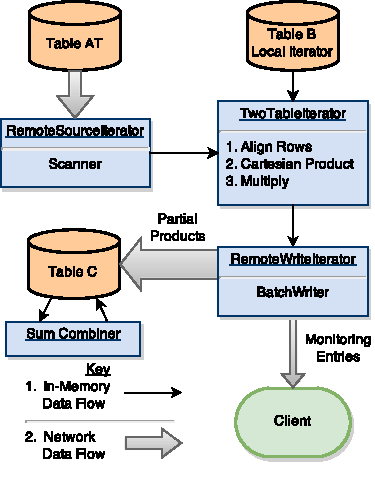
\includegraphics[width=3.0in]{TableMultIteratorStack}
%\vspace{-8pt}
\caption{Data flow through the TableMult iterator stack}
\label{fIteratorStackSpGEMM}
%\vspace{-9pt}
\end{figure}

\subsubsection{RemoteSourceIterator}
RemoteSourceIterator scans an Accumulo table
(not necessarily in the same cluster) %with the same range it is seeked to
%using credentials from the client.
using credentials passed from the client through iterator options.
%Clients pass connection information through iterator options.
%% Clients pass connection information including zookeeper hosts, timeout,
%% username and password via iterator options. %in the form of a \texttt{Map<String,String>}.
%% We leave more secure scan authentication methods to future work,
%% although only users with access to the Accumulo instance may see the password in iterator options.

We also use iterator options to specify row and column subsets, 
encoding them in a string format similar to that in D4M~\cite{kepner2012dynamic}.
Row subsets are straightforward since Accumulo uses row-oriented indexing.
Column subsets can be implemented with filter iterators
but do not improve performance since Accumulo must read every column from disk.
We encourage users to maintain a transpose table
using strategies similar to the D4M Schema~\cite{kepner2013d4m}
for cases requiring column indexing.

Multiplying table subsets is crucial for queued analytics on selected rows.
However for simpler performance evaluation, 
our experiments in Section~\ref{sPerformance} multiply whole tables.

\subsubsection{TwoTableIterator}
TwoTableIterator reads from two iterator sources, one for $\matr{A^\tr}$ and one for $\matr{B}$,
and performs the core operations of the outer product algorithm in three phases:
\begin{enumerate}
\item Align Rows.  Read entries from $\matr{A^\tr}$ and $\matr{B}$ until they advance to a matching row
or one runs out of entries. We skip non-matching rows 
since they would multiply with an all-zero row that, by Section~\ref{sMatMul}'s assumptions,
generate all zero partial products.
\item Cartesian product. Read both matching rows into an in-memory data structure. 
Initialize an iterator that emits pairs of entries from the rows' Cartesian product.
\item Multiply. Pass pairs of entries to $\otimes$ and emit results. 
\end{enumerate}

A client defines $\otimes$ by specifying a class 
that implements a multiply interface.
%which TwoTableIterator instantiates and calls. 
For our experiments we implement $\otimes$ as java.math.BigDecimal multiplication,
which guarantees correctness under large or precise real numbers.
BigDecimal decoding did not noticeably impact performance.

\subsubsection{RemoteWriteIterator}
RemoteWriteIterator writes entries to a remote Accumulo table using a BatchWriter. %created on \texttt{init}.
Entries do not have to be in sorted order because Accumulo sorts incoming entries as part of its
 ingest process. 
%% Like RemoteSourceIterator, the client passes connection information 
%% for the remote table via iterator options.

Barring extreme events such as exceptions in the iterator stack or thread death,
we designed RemoteWriteIterator to maintain correctness, such that entries generated from
its source write to the remote table once.
We accomplish this by performing all BatchWriter operations within a single function call
before ceding thread control back to the tablet server.  

A performance concern remains when multiplying a subset of the input tables' rows 
that consists of many disjoint ranges, such as one million ``singleton'' ranges spanning one row each.
It is inefficient to flush the BatchWriter before returning from each seek call, which happens once per 
disjoint scan range. %, and a known Accumulo issue could even crash the tablet server \cite{ACCUMULO-3710}.
We accommodate this case by ``transferring seek control'' %over desired row range subsets
from the tablet server to RemoteWriteIterator 
via the same strategy used in RemoteSourceIterator for seeking within an iterator.
%by encoding range objects in iterator options. %using the same technique RemoteSourceIterator uses, 
%% as opposed to the usual method of 
%% passing range objects to the %\texttt{setRanges} 
%% BatchScanner on $\matr{B}$.
%% %% RemoteWriteIterator traverses all ranges in the desired subset 
%% %% (within the tablet it runs on) in one call to seek.
%% %% %In the case of multiple tablets for table $\matr{B}$, RemoteWriteIterator running on each tablet handles 
%% %% %the portion of ranges that intersects with the range of keys in its tablet.

We include an option to BatchWrite $\matr{C}$'s transpose $\matr{C^\tr}$ in place of or alongside $\matr{C}$. 
Writing $\matr{C^\tr}$ facilitates chaining TableMults together
and maintenance of transpose indexing.

\subsubsection{Lazy $\oplus$}
We lazily sum partial products by placing a Combiner subclass implementing BigDecimal addition 
on table $\matr{C}$ at scan, minor and major compaction scopes.
Thus, $\oplus$ occurs sometime after RemoteWriteIterator writes partial products to $\matr{C}$
yet necessarily before entries from $\matr{C}$ may be seen such that we always achieve correctness.
Summation could happen when Accumulo flushes $\matr{C}$'s entries cached in memory to a new RFile, 
when Accumulo compacts RFiles together, or when a client scans $\matr{C}$. 

The key algebraic requirement for implementing $\oplus$ inside a Combiner
is that $\oplus$ must be associative and commutative.
These properties allow us to apply $\oplus$ to subsets of a result element's partial products 
and to any ordering of them, which is chaotic by outer product's nature.
If we truly had an $\oplus$ operation that required seeing all partial products at once,
we would have to either gather partial products at the client or initiate a full major compaction.

\subsubsection{Monitoring}
RemoteWriteIterator never emits entries to the client by default. 
One downside of this approach is that clients cannot precisely track progress of a TableMult operation,
which may frustrate users expecting a more interactive computing experience.
Clients could query the Accumulo monitor for read/write rates 
or prematurely scan partial products written to $\matr{C}$, but both approaches are too coarse.
%having only access to coarse Accumulo monitor rate information or partial product scans on $\matr{C}$.
%% The only information clients would have are scan and write rates from the Accumulo monitor,
%% whether a scan is running, idle or queued from the tablet server, and what partial products 
%% are written so far from scanning $\matr{C}$.

We therefore implement a monitoring option that emits a value
containing the number of entries TwoTableIterator processed
at a client-set frequency.
RemoteWriteIterator emits monitoring entries at ``safe'' points, that is,
points at which we can recover the iterator stack's state 
if Accumulo destroys, re-creates and re-seeks it.
%to a range starting from its last emitted key.
Stopping after emitting the last value in the outer product of two rows is safe 
because we place the last value's row key in the monitoring key and know, 
in the event of an iterator stack rebuild, to proceed to the next matching row.
We may succeed in stopping during an outer product 
by encoding more information in the monitoring key.
%We are also experimenting with stopping in the middle of an outer product by encoding the 
%column family and qualifier of input tables' keys in the monitoring key.


%%\subsubsection{Client API}
%% The following shows how client programs call TableMult in Java:

%% %\todo[inline]{Put Java signature of TableMult call?}

%% \definecolor{javared}{rgb}{0.6,0,0} % for strings
%% \definecolor{javagreen}{rgb}{0.25,0.5,0.35} % comments
%% \definecolor{javapurple}{rgb}{0.5,0,0.35} % keywords
%% \definecolor{javadocblue}{rgb}{0.25,0.35,0.75} % javadoc
 
%% \lstset{language=Java,
%% basicstyle=\ttfamily,
%% keywordstyle=\color{javapurple}\bfseries,
%% stringstyle=\color{javared},
%% commentstyle=\color{javagreen},
%% morecomment=[s][\color{javadocblue}]{/**}{*/},
%% numbers=left,
%% numberstyle=\tiny\color{black},
%% stepnumber=2,
%% numbersep=10pt,
%% tabsize=4,
%% showspaces=false,
%% showstringspaces=false}

%% \begin{lstlisting}

%% \end{lstlisting}


%!TEX root = Graphulo_MatrixMultiply_HPEC2015.tex

\section{Performance}
\label{sPerformance}

We evaluate TableMult with two variants of an experiment. 
First we measure the rate of computation as problem size increases.
We define problem size as number of rows in random input graphs 
represented as adjacency tables
and rate of computation as number of partial products processed per second.
Second we repeat the experiment for a fixed size problem with all tables split into two tablets,
allowing Accumulo to scan and write to them in parallel.

%% We evalutate our TableMult implementation with a weak scaling experiment,
%% measuring rate of computation as problem size increases.
%% We define problem size as the number of nodes in random input graphs
%% and rate of computation as the number of partial products processed per second.  
%% We also perform the same tests when input and output tables
%% are split into two tablets each, which allows Accumulo to scan and write to them in parallel.

%Ideally we would include run our tests on more than two tablets to truly test strong scaling, 
%but such tests are infeasible given the laptop's capabilities.

We compare Graphulo TableMult performance to D4M~\cite{kepner2012dynamic} as a baseline because 
a user with one client machine's best alternative is reading input graphs from Accumulo, 
multiplying them at the client, and inserting the result back into Accumulo.
%D4M well represents the best of Accumulo client algorithms. has excelled at high scan and ingest rates and has 

D4M stores tables as Associative Array objects in \matlab{}.  
Because Assoc Array multiplication runs fast
by calling \matlab{}'s in-memory sparse matrix functions, 
D4M bottlenecks on reading data from Accumulo and especially on writing back results,
despite its capacity for high speed Accumulo reads and writes~\cite{kepner2014achieving}.
We consequently expect TableMult to outperform D4M 
because TableMult avoids transferring data out of Accumulo for processing. 

We also expect TableMult to succeed on larger graph sizes than D4M because TableMult
uses a streaming outer product algorithm that does not store input tables in memory.
An alternative D4M implementation would mirror TableMult's streaming outer product algorithm,
enabling D4M to run on larger problem sizes at potentially worse performance.
We therefore imagine the whole-table D4M algorithm as an upper bound on the best performance 
achievable when multiplying Accumulo tables outside Accumulo's infrastructure.

We use the Graph500 unpermuted power law graph generator \cite{bader2006designing} 
to create random input tables,
 %also used in 100M insert/sec paper
such that the first row has high degree (number of columns) 
%The generator creates graphs with a power law structure, such that the first vertex has high degree
and subsequent rows exponentially decrease in degree.
The generator takes SCALE and EdgesPerVertex parameters, creating graphs with 2\textsuperscript{SCALE} 
rows and EdgesPerVertex $\times$ 2\textsuperscript{SCALE} entries.
We fix EdgesPerVertex to 16 and use SCALE to vary problem size. 

%We multiply the transpose of the first table with the second table in our tests.
The following procedure outlines our performance experiment for a given SCALE and either one or two tablets.
\begin{enumerate}
\item Generate two graphs with different random seeds and insert them into Accumulo as adjacency tables via D4M.
\item In the case of two tablets, identify an optimal split point for each input graph
and set the input graphs' table splits equal to that point.
``Optimal'' here means a split point that evenly divides an input graph into two tablets.
\item \label{ePreSplit1} Create an empty output table. For two tablets, pre-split it with 
an optimal input split position recorded from a previous multiplication run.
%% the first input table's split.
%% The split will not be optimal for the output table because the matrix product has a different degree distribution 
%% than that of the input tables, but it is close enough for the purposes of our test.
\item \label{ePreSplit1Compact} Compact the input and output tables 
so that Accumulo redistributes the tables' entries into the assigned tablets.
\item Run and time Graphulo TableMult multiplying the transpose of the first input table with the second.
\item Create, pre-split and compact a new result table for the D4M comparison 
as in step~\ref{ePreSplit1} and~\ref{ePreSplit1Compact}.
\item Run and time the D4M equivalent of TableMult:
 \begin{enumerate}
 \item Scan both input tables into D4M Associative Array objects in \matlab{} memory.
 \item Convert the string values from Accumulo into numeric values for each Associative Array.
 \item Multiply the transpose of the first Associative Array with the second.
 \item Convert the result Associative Array back to String values and insert them into Accumulo.
 \end{enumerate}
\end{enumerate}

%\subsection{Environment}
We conducted the experiments on a Ubuntu Linux laptop with 16GB RAM and two dual-core Intel i7 processors%at 3GHz
. Using single-instance Accumulo 1.6.1, Hadoop 2.6.0 and ZooKeeper 3.4.6,
%On top of Hadoop 2.6.0 and ZooKeeper 3.4.6,
we allocated 2GB of memory to an Accumulo tablet server initially
(allowing growth in 500MB steps),
1GB for native in-memory maps and 256MB for data and index cache.


We chose not to use more than two tablets per table because more threads would run
than the laptop could handle.  Each additional tablet can potentially add the following threads:
\begin{enumerate}
\item Table $\matr{A}^\tr$ server-side scan thread;
\item Table $\matr{A}^\tr$ client-side scan thread,

$\quad$ running from RemoteSourceIterator;
\item Table $\matr{B}$ server-side scan/multiply thread,

$\quad$ running a TableMult iterator stack;
\item Table $\matr{B}$ client-side scan thread, 

$\quad$ running from the initiating client, mostly idle;
\item Table $\matr{C}$ server-side write thread;
\item Table $\matr{C}$ client-side write thread,

$\quad$ running from RemoteWriteIterator; and
\item Table $\matr{C}$ server-side minor compaction threads,

$\quad$ running with a Combiner implementing $\oplus$.
\end{enumerate}

\begin{figure}[t]
%\vspace{-6pt}
\centering
\includegraphics[width=\linewidth]{TableMultRate}
\caption{TableMult Processing Rate vs. Input Table Size}
\label{fTableMultPerf}
%\vspace{-4pt}
\end{figure}

We show table $\matr{C}$ sizes and experiment timings in Table~\ref{tResultsParams}
and plot them in Figure~\ref{fTableMultPerf}.
We could not run the D4M comparison past SCALE 15 because $\matr{C}$ does not fit in memory.

For the scaled problem, the best results we could achieve are flat horizontal lines, 
indicating that we maintain the same level of operations per second as problem size increases.
%Graphulo roughly achieves weak scaling, although the two-tablet Graphulo curve shows instability.

One reason we see a downward rate trend at larger problem sizes is that Accumulo
needs to minor compact table $\matr{C}$ in the middle of a TableMult. 
The compactions trigger flushes to disk along with 
the $\oplus$ Combiner that sums partial products written to $\matr{C}$ so far, 
neither of which we include 
in rate measurements. % (in partial products per second).
%% Thus, one explanation for the rate decrease is that 
%% our rate measurements (in partial products per second) do not include summing 
%% and disk flush operations Accumulo performs during minor compaction.

For the fixed size problem, the best results we could achieve are two-tablet rates at
double the one-tablet rates at every problem size.
Our experiment shows that Graphulo two-tablet rates perform up to 1.5x better
than one-tablet rates at lower SCALEs. %with degraded performance at higher SCALEs.  
We attribute TableMult's shortfall to high processor contention for the laptop's four cores as a result of 
the 14 threads that may run concurrently when each table has two tablets; in fact,
processor usage hovered near 100\% for all four cores throughout the two-tablet experiments.
We expect better scaling when running our experiment 
in larger Accumulo clusters that can handle more degrees of parallelism.

%Odd factor: OS frequently killed the Accumulo garbage collector.

\begin{table*}[tb]
%\vspace{-0.5em}
\centering                                                                                                           
\caption{Output Table $\matr{C}$ Sizes and Experiment Timings}% plotted in Figure~\ref{fTableMultPerf}}
\label{tResultsParams}
\begin{threeparttable}[c]
\begin{tabular}{r|ll|ll|ll|ll|ll}
 & \multicolumn{2}{c|}{Entries in Table $\matr{C}$} & \multicolumn{2}{c|}{Graphulo 1 Tablet} & \multicolumn{2}{c|}{D4M 1 Tablet} & \multicolumn{2}{c|}{Graphulo 2 Tablets} & \multicolumn{2}{c}{D4M 2 Tablets} \\
SCALE & PartialProducts & AfterSum & Time (s) & Rate (pp/s) & Time (s) & Rate (pp/s) & Time (s) & Rate (pp/s) & Time (s) & Rate (pp/s) \\             
\hline
10 & \num{804989.000} & \num{269404.000} & \num{2.865} & \num{281012.707} & \num{3.018} & \num{266771.720} & \num{2.022} & \num{398174.309} & \num{2.804} & \num{287060.355} \\             
\hline                                                                                                                                                                                                          
11 & \num{2361580.000} & \num{814644.000} & \num{7.758} & \num{304413.622} & \num{8.803} & \num{268259.547} & \num{5.189} & \num{455121.509} & \num{8.718} & \num{270898.575} \\            
\hline                                                                                                                                                                                                          
12 & \num{6816962.000} & \num{2430381.000} & \num{21.984} & \num{310090.248} & \num{26.601} & \num{256270.986} & \num{16.307} & \num{418039.002} & \num{26.182} & \num{260366.279} \\       
\hline                                                                                                                                                                                                          
13 & \num{19111689.000} & \num{7037007.000} & \num{63.969} & \num{298766.256} & \num{150.475} & \num{127009.402} & \num{48.623} & \num{393059.423} & \num{144.156} & \num{132575.978} \\    
\hline                                                                                                                                                                                                          
14 & \num{52656204.000} & \num{20029427.000} & \num{181.506} & \num{290106.916} & \num{579.243} & \num{90905.237} & \num{136.025} & \num{387107.096} & \num{559.271} & \num{94151.551} \\   
\hline                                                                                                                                                                                                          
15 & \num{147104084.000} & \num{58288789.000} & \num{502.864} & \num{292532.774} & \num{2510.389} & \num{58598.135} & \num{393.573} & \num{373765.880} & \num{2559.243} & \num{57479.523} \\
\hline                                                                                                                                                                                                          
16 & \num{400380031.000} & \num{163481262.000} & \num{1390.612} & \num{287916.484} &  &  & \num{1178.111} & \num{339849.273} &  &  \\                                                               
\hline                                                                                                                                                                                                          
17 & \num{1086789275.000} & \num{459198683.000} & \num{4064.990} & \num{267353.526} &  &  & \num{3699.671} & \num{293752.983} &  &  \\                                                              
\hline                                                                                                                                                                                                          
18 & %2.94 \times 10^9%
%\num{2937549526} 
& \num{1280878452.000} & \num{12148.744} & \num{241798.621} &  &  & \num{11369.009} & \num{258382.204} &  &  \\
\end{tabular}
%\begin{tablenotes}
%\tnote{1}
%\item [a] nnz($\matr{C}$) is the number of elements in output table $\matr{C}$ after all partial products sum together.
%\end{tablenotes}
\end{threeparttable}
\vspace{-1.5em}
\end{table*}

%!TEX root =SpGEMM_Accumulo_HPEC.tex

\section{Discussion}
\label{sDiscussion}

\subsection{Related Work} %Analogy to MapReduce with Accumulo Scanners, Iterators and BatchWriters:
%\todo[inline]{Cannon's algorithm, other SpGEMM}
Bulu\c{c} and Gilbert studied message passing algorithms for SpGEMM
such as Sparse SUMMA, most of which use 2D block decompositions \cite{buluc2012parallel}.
Unfortunately, 2D decompositions are difficult in Accumulo 
and message passing even more so.
In this work, we use Accumulo's native 1D decomposition along rows 
and do not rely on tablet server communication
apart from shuffling partial products of $\matr{C}$ via BatchWriters.


Our outer product method could have been implemented in MapReduce %x\cite{dean2008mapreduce} 
on Hadoop or its successor YARN \cite{vavilapalli2013apache}.
There is a natural analogy from TableMult to MapReduce:
the map phase scans rows from $\matr{A^\tr}$ and $\matr{B}$
and generates a list of partial products from TwoTableIterator;
the shuffle phase sends partial products to correct tablets of $\matr{C}$ via BatchWriters;
the reduce phase sums partial products using Combiners.
Examining the conditions on which MapReduce 
reading from and writing to Accumulo's RFiles directly
can outperform Accumulo-only solutions
is worthy future work.

%TableMult Design Alternatives
%% A common Accumulo pattern is to %run multiple clients %that scan disjoint and continuous table sections in parallel.
%% scan and write from multiple clients in parallel.
%% %In fact, 
%% The high insert rates of \cite{kepner2014achieving}
%% were obtained using 
%% parallel clients aware of tablet locations.
%% %% Kepner et al used parallel clients and tablet location info
%% %% to insert at record-setting rates \cite{kepner2014achieving}.

A common Accumulo pattern is to 
scan and write from multiple clients in parallel;
in fact, researchers obtained 
considerably high insert rates using parallel client strategies \cite{kepner2014achieving}.
We chose to build Graphulo as a service within Accumulo
instead of assuming multiple client capability,
such that Graphulo is as accessible as possible to diverse client environments.

The strategy in \cite{kepner2014achieving} 
also used %information on tablet assginment to tablet servers
%physical 
tablet location information
to determine where clients could write locally.
Knowing tablet-to-tablet-server assignment could likewise aid Graphulo, 
not only to minimize network traffic
but also
 to partly eliminate Apache Thrift RPC serialization,
which prior work has shown is a bottleneck for scans % writes?
when iterator processing is light \cite{sawyer2013understanding}.
%Enhancing Accumulo for non-Thrift, local access may 
Such an enhancement would access a local tablet server by method call 
in place of Scanners and BatchWriters.
%use a new access inter-process chanel 
%optimized for 

%% %% In order to make Graphulo as accessible to client environments %configurations
%% %% as possible, we built Graphulo as a service within Accumulo 
%% %% instead of assuming multiple client capabilities.
%% %%% We avoid the multiple client pattern because it increases client software complexity,
%% %%% whereas we aim for a service within Accumulo that works for any client.
%% As described in \cite{sawyer2013understanding}, 
%% table scans that do not perform significant iterator processing
%% bottleneck on communication overhead at the client due to Apache Thrift serialization.
%% %% %filtering or other server-side computation 
%% %% Future work may eliminate this bottleneck by 
%% %% avoiding 
%% % avoid RPCs
%% % local tablet location information
%% %We gain a chance to eliminate Thrift overhead %by moving computation to the server,
%% Future work may eliminate Thrift overhead
%% for scans and writes to tablets located on the same tablet server.
%% %though the current version does not do so because standard Scanners and BatchWriters serialize as clients would.

\subsection{Design Alternative: Inner-Outer Product Hybrid}

%bridge inner and outer product
It is worth reconsidering the inner product method from our initial design
because it has an opposite performance profile as 
Figure~\ref{fInnerOuterSpectrum}'s left and right depict: 
inner product bottlenecks on scanning whereas outer product bottlenecks on writing.
At the expense of multiple passes over input matrices, inner product emits 
partial products in order and immediately pre-summable,
%more efficiently in that emitted entries are in order and partial products can sum immediately, 
reducing the number of entries written to Accumulo to the minimum possible.
Outer product reads inputs in a single pass
but emits entries out of order and has little chance to pre-sum, 
instead writing individual partial products to $\matr{C}$.
Table~\ref{tResultsParams} quantifies that outer product writes
2.5 to 3 times more entries than inner product for power law inputs.
In the worst case, multiplying a fully dense $n \times m$ with an $m \times p$ matrix,
outer product emits $m$ times more entries than inner product.



%LRU cache enables the bridge
Is it possible to blend inner and outer product SpGEMM methods,
choosing a middle point in Figure~\ref{fInnerOuterSpectrum}
with equal read and write bottlenecks for overall greater performance?
In the following generalization, 
partition parameter $P$ varies behavior between
inner product at $P=n$ and outer product at $P=1$:

\removelatexerror
\begin{algorithm}[H]
\vspace{\algspace}
\SetKwBlock{fore}{for}{} 
\SetKw{emit}{emit}
\fore($l = 1\col P$){
\fore($k = 1\col m$){
\fore({$i = \left( \floor*{\dfrac{(l-1)n}{P}}+1 \right) \col \floor*{\dfrac{ln}{P}}$}){
\fore($j = 1\col p$){
%\vspace{4pt}
\emit{$ \matr{A}(i,k) \otimes \matr{B}(k,j)$}
}}}}
\vspace{\algspace}
\end{algorithm}

The hybrid algorithm runs $P$ passes through $\matr{B}$,
each of which has write locality to a vertical partition of $\matr{C}$ of size $\ceil{n / P}$.
Pre-summing ability likewise varies inversely with $P$, 
though actual pre-summing depends on
$\matr{A}$ and $\matr{B}$'s  sparsity distribution
as well as how many positions of $\matr{C}$ the TableMult iterators cache.
Figure~\ref{fInnerOuterSpectrum}'s center depicts the $P=2$ case.

\begin{figure}[htb]
\vspace{-4pt}
\centering
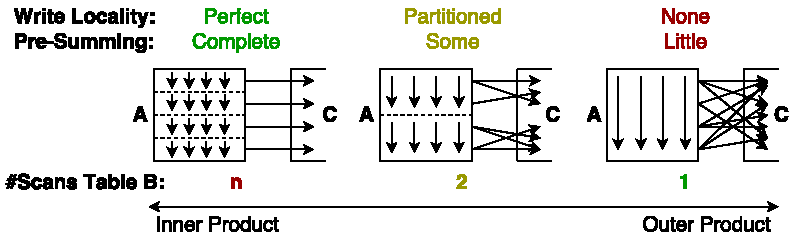
\includegraphics[width=\linewidth]{InnerOuterSpectrum}
\vspace{-14pt}
\caption{Tradeoffs between Inner and Outer Product}
\label{fInnerOuterSpectrum}
%\vspace{-2pt}
\end{figure}


A challenge for any hybrid algorithm is mapping it to Accumulo infrastructure.
We chose outer product because it more naturally fits Accumulo, 
using iterators for one-pass streaming computation, 
BatchWriters to handle unsorted entry emission and Combiners to defer summation.
The above hybrid algorithm resembles 2D block decompositions,
and so maximizing its performance may be challenging 
given limited data layout control and unknown data distribution.
%Further investigation is future work.
%Hybrid solutions might consider locality groups or transpose tables to enable column-oriented scanning
%and the distribution of tablets to tablet server cost modeling to 
%% We may realize greater performance by considering data placement among tablet servers, 
%% but such a consideration would require accessing and perhaps manipulating
%% Accumulo's internal state and non-public API.
%% We suggest this paper's approach as a balance between top performance and implementation stability.

Nevertheless, possible design criteria are to minimize $P$ in order to minimize passes through $\matr{B}$,
while also choosing $P$ large enough so that $\ceil{\frac{np}{P}}$ entries fit in memory
(dense matrix worst case), which guarantees complete pre-summing.
The latter criterion may be relaxed with decreasing matrix density.


\subsection{TableMult in Algorithms}
Several optimization opportunities exist for TableMult as a primitive in larger algorithms.
Suppose we have a program $\matr{E} = \matr{AB}; \matr{F} = \matr{CD}; \matr{G} = \matr{EF}$.
We would save two round trips to disk if we could mark $\matr{E}$ and $\matr{F}$ as 
``temporary tables,'' i.e. tables intermediate to an algorithm that should be held in memory 
and not written to Hadoop if possible.

A \emph{pipelining} optimization streams entries from a TableMult 
to computations taking its result as input. 
Outer product pipelining is difficult
because it cannot guarantee writing every partial product for a particular element 
 to $\matr{C}$ until it finishes,
whereas inner product's complete pre-summing emits elements ready for downstream use.
More ambitiously, \emph{loop fusion} merges iterator stacks 
for successive computations into one. 

Optimizing computation on NoSQL databases is challenging in the general case because
NoSQL databases mostly exclude query planner features 
customary of SQL databases in exchange for raw performance.
% and simplicity of implementation
NewSQL databases aim in part to achieve the best of both worlds---performance and query planning \cite{grolinger2013data}.
We aspire to make a small step for Accumulo in the direction of NewSQL with current Graphulo research.






\section{Conclusions}
\label{sConclusions}

In this work we showcase the design of TableMult, a Graphulo implementation of the 
SpGEMM GraphBLAS linear algebra kernal server-side on Accumulo tables.
We compare inner and outer approaches and show how outer product 
better fits Accumulo's iterator model.
Performance experiments show good weak scaling and hint at strong scaling,
although repeating experiments on a larger cluster is necessary to confirm.

Current research in addition to topics from Section~\ref{sDiscussion}'s discussion, 
is to implement the remaining GraphBLAS kernels 
and develop algorithms calling them, % atop the Graphulo library,
ultimately delivering a Graphulo linear algebra library 
as a pattern for server-side computation
to the Accumulo community.


%\begin{figure}[!t]
%\centering
%\includegraphics[width=2.5in]{myfigure}
% where an .eps filename suffix will be assumed under latex,
% and a .pdf suffix will be assumed for pdflatex; or what has been declared
% via \DeclareGraphicsExtensions.
%\caption{Simulation Results}
%\label{fig_sim}
%\end{figure}

% Note that IEEE typically puts floats only at the top, even when this
% results in a large percentage of a column being occupied by floats.


% An example of a double column floating figure using two subfigures.
% (The subfig.sty package must be loaded for this to work.)
% The subfigure \label commands are set within each subfloat command, the
% \label for the overall figure must come after \caption.
% \hfil must be used as a separator to get equal spacing.
% The subfigure.sty package works much the same way, except \subfigure is
% used instead of \subfloat.
%
%\begin{figure*}[!t]
%\centerline{\subfloat[Case I]\includegraphics[width=2.5in]{subfigcase1}%
%\label{fig_first_case}}
%\hfil
%\subfloat[Case II]{\includegraphics[width=2.5in]{subfigcase2}%
%\label{fig_second_case}}}
%\caption{Simulation results}
%\label{fig_sim}
%\end{figure*}
%
% Note that often IEEE papers with subfigures do not employ subfigure
% captions (using the optional argument to \subfloat), but instead will
% reference/describe all of them (a), (b), etc., within the main caption.


% An example of a floating table. Note that, for IEEE style tables, the
% \caption command should come BEFORE the table. Table text will default to
% \footnotesize as IEEE normally uses this smaller font for tables.
% The \label must come after \caption as always.
%
%\begin{table}[!t]
%% increase table row spacing, adjust to taste
%\renewcommand{\arraystretch}{1.3}
% if using array.sty, it might be a good idea to tweak the value of
% \extrarowheight as needed to properly center the text within the cells
%\caption{An Example of a Table}
%\label{table_example}
%\centering
%% Some packages, such as MDW tools, offer better commands for making tables
%% than the plain LaTeX2e tabular which is used here.
%\begin{tabular}{|c||c|}
%\hline
%One & Two\\
%\hline
%Three & Four\\
%\hline
%\end{tabular}
%\end{table}


% Note that IEEE does not put floats in the very first column - or typically
% anywhere on the first page for that matter. Also, in-text middle ("here")
% positioning is not used. Most IEEE journals/conferences use top floats
% exclusively. Note that, LaTeX2e, unlike IEEE journals/conferences, places
% footnotes above bottom floats. This can be corrected via the \fnbelowfloat
% command of the stfloats package.

% conference papers do not normally have an appendix


% use section* for acknowledgement
%% \section*{Acknowledgment}

%% The authors wish to thank the entire Graphulo team at MIT CSAIL and
%% MIT Lincoln Laboratory. We also thank the GraphBLAS contributors and
%% National Science Foundation for their generous ongoing support of this program.

% trigger a \newpage just before the given reference
% number - used to balance the columns on the last page
% adjust value as needed - may need to be readjusted if
% the document is modified later
%\IEEEtriggeratref{8}
% The "triggered" command can be changed if desired:
%\IEEEtriggercmd{\enlargethispage{-5in}}

% references section

% can use a bibliography generated by BibTeX as a .bbl file
% BibTeX documentation can be easily obtained at:
% http://www.ctan.org/tex-archive/biblio/bibtex/contrib/doc/
% The IEEEtran BibTeX style support page is at:
% http://www.michaelshell.org/tex/ieeetran/bibtex/
%\bibliographystyle{IEEEtran}
% argument is your BibTeX string definitions and bibliography database(s)
%\bibliography{IEEEabrv,../bib/paper}
%
% <OR> manually copy in the resultant .bbl file
% set second argument of \begin to the number of references
% (used to reserve space for the reference number labels box)


%\begin{thebibliography}{1}
%
%\bibitem{NIST}
%P.~Mell and T.~Grace, \emph{The NIST Definition of Cloud Computing},
%NIST Special Publication 800-145
%
%\end{thebibliography}

\bibliographystyle{IEEEtran}
\balance
\bibliography{10_bibliography}

%\appendix
%\section*{Performance Numbers}


\end{document}


